\documentclass[a4paper,12pt]{article}

\usepackage[cp1251]{inputenc}
\usepackage[russian]{babel}
\usepackage[T2A]{fontenc}
\usepackage{float}
\usepackage{subfigure}

\usepackage{booktabs}

\usepackage{graphicx}

\usepackage{amsthm}
\usepackage{import}

\usepackage{indentfirst}

\usepackage[labelsep=period,labelfont=bf,figurename={Рис.},figurewithin=none]{caption}

\usepackage{wrapfig}

\usepackage{amsmath}

\usepackage{amssymb}

\usepackage[a4paper,top=1.3cm,bottom=2cm,left=1.5cm,right=1.5cm,marginparwidth=0.75cm]{geometry}

\begin{document}

\begin{titlepage}
\begin{center}
    {\large МОСКОВСКИЙ ФИЗИКО-ТЕХНИЧЕСКИЙ ИНСТИТУТ (НАЦИОНАЛЬНЫЙ ИССЛЕДОВАТЕЛЬСКИЙ УНИВЕРСИТЕТ)}
\end{center}

\begin{center}
    {\large Физтех-школа радиотехники и компьютерных технологий}
\end{center}

\vspace{3.5cm}

\begin{center}
    
\includegraphics[width=0.4\linewidth]{img/hv_full.png}
\end{center}

\vspace{0.1cm}

{\huge
\begin{center}
    {\bf Лабораторная работа 2.3.1}\\
    Получение и измерение вакуума
\end{center}
}

\vspace{2cm}

\begin{flushright}
{\LARGE Автор:\\ Григорьев Даниил \\
\vspace{0.2cm}
Б01-407}
\end{flushright}

\vspace{3.5cm}
\begin{center}
    Долгопрудный 2025
\end{center}
\end{titlepage}

\section{Аннотация}
    \paragraph{Цель работы:} 1) измерение объемов форвакуумной и высоковакуумной
    частей установки;
    2) определение скорости откачки системы в стационарном режиме,
    а также по ухудшению и улучшению вакуума.
    \paragraph{В работе используются:} вакуумная установка с манометрами: масляным,
    термопарным и ионизационным.

\section{Теоретическая часть}
    \subsection{Процесс откачки}

    Пусть W --- объем газа, удаляемого из
    сосуда при данном давлении за единицу времени, $Q_i$ для различных значений
    $i$ обозначим различные притоки газа в сосуд (в единицах $PV$), такие как
    течи извне $Q_\text{и}$, десорбция с поверхностей внутри сосуда
    $Q_\text{д}$, обратный ток через насос $Q_\text{н}$. Тогда имеем:
    \begin{equation} -VdP = \left(PW - \sum Q_i\right)dt \end{equation} При
    достижении предельного вакуума устанавливается $P_{\text{пр}}$, и $dP = 0$.
    В таком случае: \begin{equation} W = \frac{\sum Q_i}{ P_{\text{пр}}}
    \end{equation} Поскольку обычно $Q_\text{и}$ постоянно, а $Q_\text{н}$ и
    $Q_\text{д}$ слабо зависят от времени, также считая постоянной W, можем
    проинтегрировать (1) и получить: \begin{equation} P - P_{\text{пр}} = (P_0 -
    P_{\text{пр}})\exp\left(-\frac{W}{V}t\right) \label{exp} \end{equation}
    Полная скорость откачки $W$, собственная скорость откачки насоса
    $W_{\text{н}}$ и проводимости элементов системы $C_1, C_2,\;\ldots$
    соотносятся согласно формуле (4), и это учтено в конструкции установки.
    \begin{equation} \frac{1}{W} = \frac{1}{W_\text{н}} + \frac{1}{C_1} +
    \frac{1}{C_2} + \ldots \end{equation}

\subsection{Течение газа через трубу}

	Характер течения газа существенно зависит от соотношения между размерами
	системы и длиной свободного пробега молекул. При атмосферном и форвакуумном
	давлениях  длина свободного пробега меньше диаметра трубок, и течение газа
	определяется его вязкостью, т.е. взаимодействием молекул. При переходе к
	высокому вакууму столкновения молекул между собой начинают играть меньшую
	роль, чем соударения со стенками.

	Для количества газа, протекающего через трубу длины $l$ и радиуса $r$ в
	условиях высокого вакуума, справедлива формула: \begin{equation}
	\frac{d(PV)}{dt} = \frac{4}{3}r^3\sqrt{\frac{2\pi RT}{\mu}}\cdot\frac{P_2 -
	P_1}{l} \label{kap} \end{equation} Если труба соединяет установку с
    насосом, то
	давлением $P_1$ у его конца можно пренебречь. Давление в сосуде $P = P_2$.
	Тогда пропускная способность трубы: \begin{equation} C_\text{тр} =
	\left(\frac{dV}{dt}\right)_\text{тр} = \frac{4r^3}{3l}\sqrt{\frac{2\pi
	RT}{\mu}} \label{ty} \end{equation}

\section{Экспериментальная установка}

    Установка изготовлена из стекла,
	и состоит из форвакуумного баллона (ФБ), высоковакуумного диффузионного
	насоса (ВН), высоковакуумного баллона (ВБ), масляного (М) и ионизационного
	(И) манометров, термопарных манометров ($\text{М}_1$ и $\text{М}_2$),
	форвакуумного насоса (ФН) и соединительных кранов ($\text{K}_1,
	\text{K}_2,\; \ldots \;\text{K}_6$) (Рис. 1). Кроме того, в
	состав установки входят: реостат и амперметр для регулирования тока
	нагревателя диффузионного насоса.

    \begin{figure}[H]
        \centering
        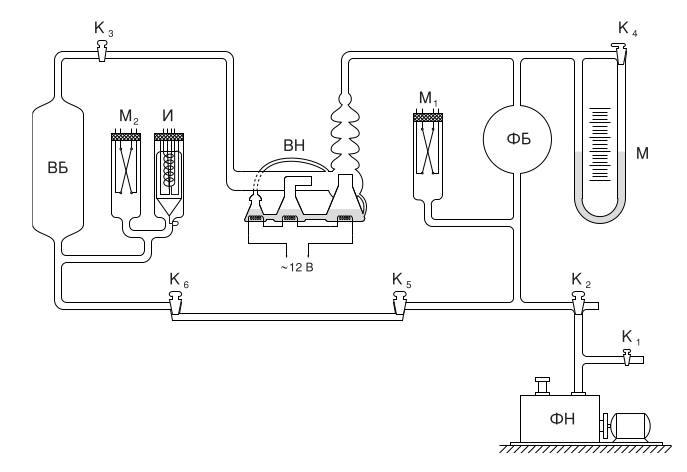
\includegraphics[scale=2]{img/stand.png}
        \caption{Схема экспериментальной установки}
        \label{facility}
    \end{figure}

\section{Ход работы}

\subsection{Определение объема форвакуумной и высоковакуумной частей
    установки}
    \begin{enumerate}
        \item Атмосферное давление равно $P_{\text{A}} = (752\pm1)$ торр.
        \item Впустим в установку атмосферный воздух через краны К1 и К2.
        \item Закроем краны К5 и К6, запрем $V_{\text{зап}} = 50$ см$^3$
        воздуха.
        \item Закроем краны К1 и К2, включим форвакуумный насос. Подключим
        установку к форвакуумному насосу краном К2 и откачаем ее до давления
        $10^{-2}$ торр.
        \item Повернув рукоятку крана К2, отсоединим установку от форвакуумного
        насоса. Откроем кран К1.
        \item Перекрыв К3, отделим ВБ от ФБ.
        \item Закроем К4.
        \item Откроем К5, измерим уровень масла слева и справа, которые
        дадут нам давление $P_1$.
        Из закона Бойля-Мариотта $V_{\text{фв}} = V_{\text{зап}}P_{\text{A}}/
        P_1$.
        \item Аналогичным методом измерим объем $V_{\text{вв}}$, открыв кран
        К3.
        \item Результаты первого измерения в таблице 1.
        Погрешность измерения уровня примем $\Delta h = 0{,}1$ см.
        \begin{table}[H]
            \centering
            \begin{tabular}{|c|c|c|c|c|c|}
                \hline
                $h_1$, см & $h_2$, см & $P_1$, торр & $h_3$, см & $h_4$, см & $P_2$, торр \\\hline
                35{,}0    & 15{,}0    & 13{,}0      & 31{,}6    & 18{,}8    & 8{,}3      \\\hline
            \end{tabular}
            \caption{Таблица первых показаний масляного манометра.}
        \end{table}

        Сотрудник лаборатории сразу понял, что измерения неверны, поэтому измерим второй раз, более внимательно. Результаты в таблице 2.

        \begin{table}[H]
            \centering
            \begin{tabular}{|c|c|c|c|c|c|}
                \hline
                $h_1$, см & $h_2$, см & $P_1$, торр & $h_3$, см & $h_4$, см & $P_2$, торр \\\hline
                38{,}3    & 11{,}3    & 18{,}6      & 33{,}7    & 16{,}3    & 11{,}8      \\\hline
            \end{tabular}
            \caption{Таблица вторых показаний масляного манометра.}
        \end{table}
        Расхождения в измерениях скорее всего связаны с тем,
        что в первом случае при снятии измерений мы поторопились и не дождались равновесного положения жидкости в масляном манометре.
        \item Получим $V_{\text{фв}} = (2139\pm40)$ см$^3$,
        $V_{\text{вв}} = (1180\pm30)$ см$^3$. Относительная погрешность может
        быть вычислена в обоих случаях как $\varepsilon_V = \varepsilon_P +
        \varepsilon_{P_{\text{A}}}$. $\varepsilon_{V_{\text{фв}}} = 0{,}2$,
        $\varepsilon_{V_{\text{вв}}} = 0{,}3$.

    \end{enumerate}

 \subsection{Получение высокого вакуума и измерение скорости откачки}
    \begin{enumerate}
        \setcounter{enumi}{11}
        \item Установим ток в лампе $I_0 = 0{,}6$ А.
        \item После того, как давление упало ниже $3\cdot 10^{-2}$ торр,
        закроем К6 и установим ток $I_{\text{max}} = 1{,}29$ А для нагревания
        масла.
        \item Когда давление достигнет $10^{-3}$ торр, включим ионизационный
        манометр.
        \item По достижении $1{,}6\cdot 10^{-4}$ торр начнем дегазацию.
        \item Получаем предельное давление $P_{\text{пр}} = 7{,}5\cdot 10^{-5}$
        торр.
        \item Остановим откачку и откроем кран К3. Снимем зависимость $P(t)$
        в процессе ухудшения, а затем в процессе улучшения вакуума.
        \item Все результаты представим на графиках:

        \begin{figure}[h!]
            \centering
            \begin{minipage}{0.45\textwidth}
                \centering
                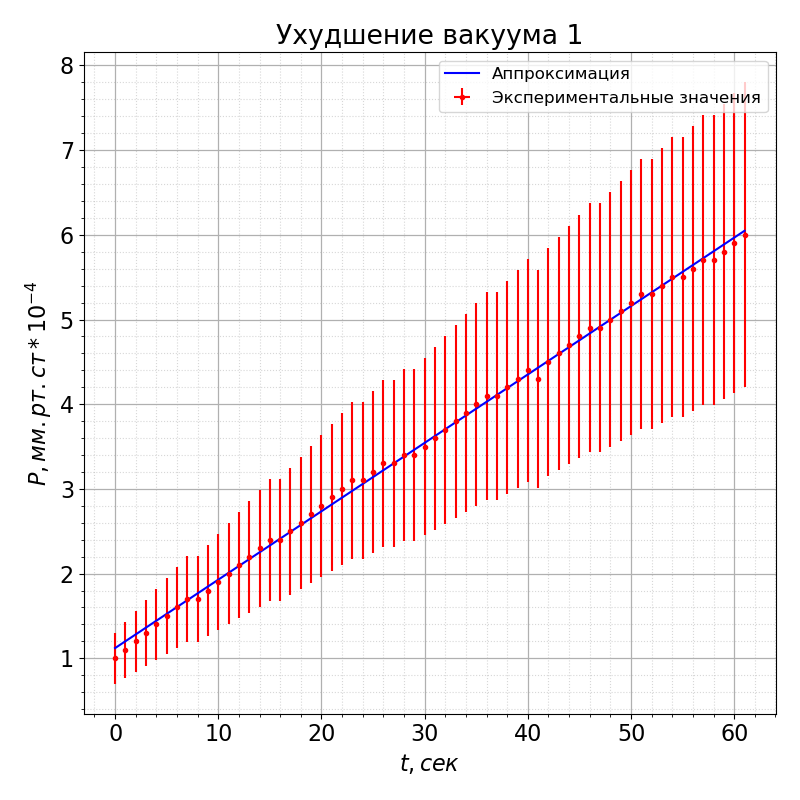
\includegraphics[width=1\linewidth]{img/rise1.png}
                \captionof{figure}{Ухудшение вакуума 1}
                \label{rise1}
            \end{minipage}
            \begin{minipage}{0.45\textwidth}
                \centering
                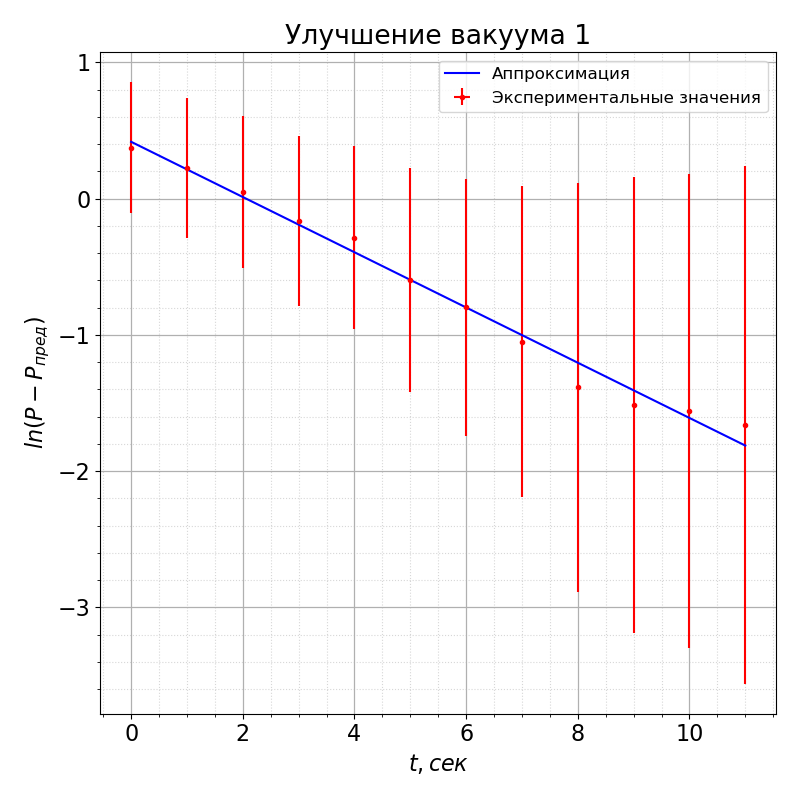
\includegraphics[width=1\linewidth]{img/fall1.png}
                \captionof{figure}{Улучшение вакуума 1}
                \label{fall1}
            \end{minipage}
        \end{figure}

        \begin{figure}[h!]
            \centering
            \begin{minipage}{0.45\textwidth}
                \centering
                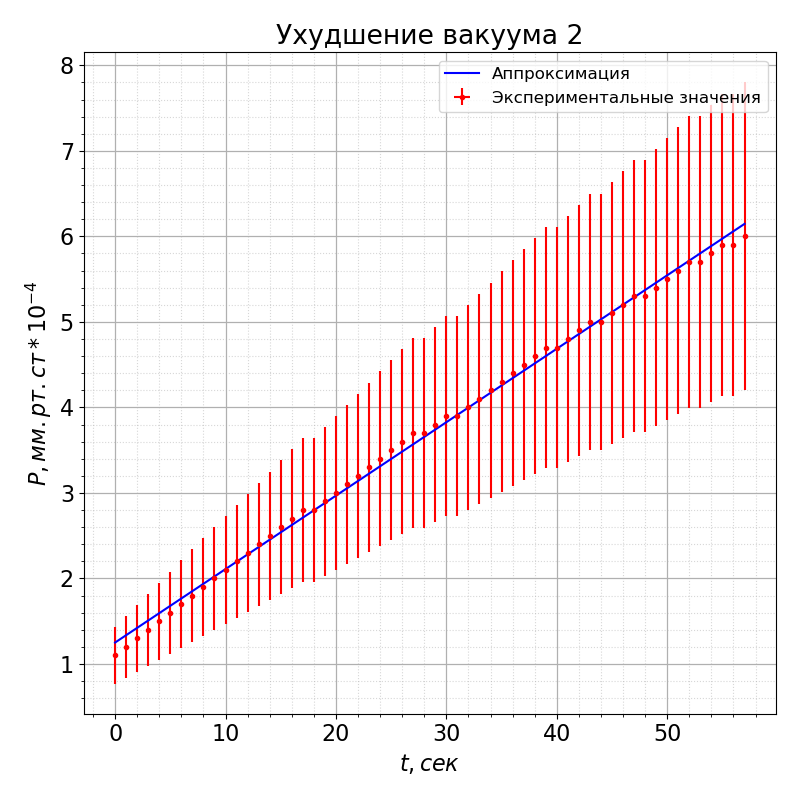
\includegraphics[width=1\linewidth]{img/rise2.png}
                \captionof{figure}{Ухудшение вакуума 2}
                \label{rise2}
            \end{minipage}
            \begin{minipage}{0.45\textwidth}
                \centering
                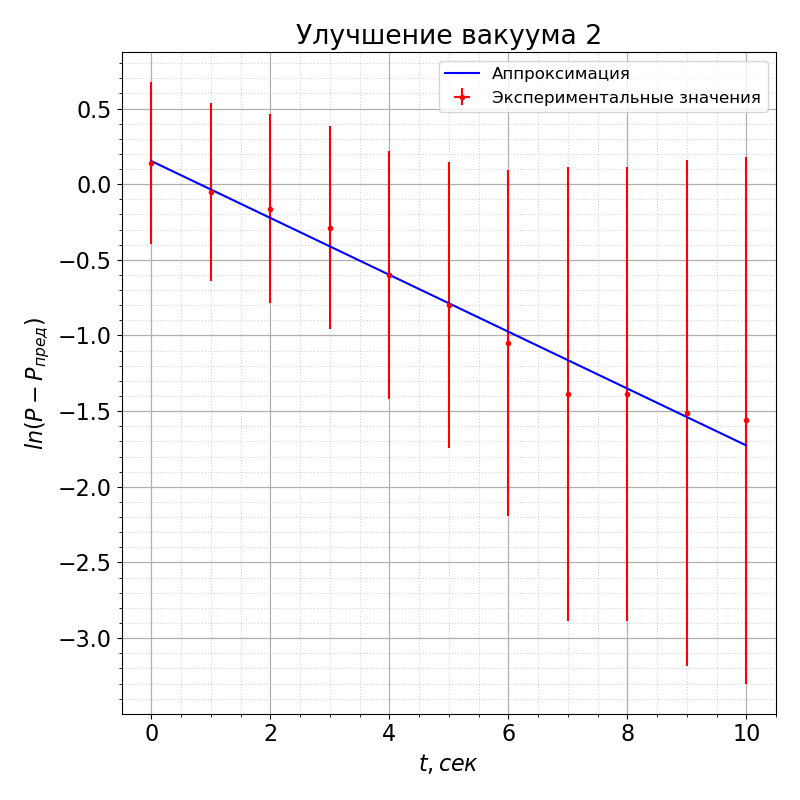
\includegraphics[width=1\linewidth]{img/fall2.png}
                \captionof{figure}{Улучшение вакуума 2}
                \label{fall2}
            \end{minipage}
        \end{figure}

    Из графиков $\ref{fall1}$ и \ref{fall2} по МНК получаем коэффициенты прямых:

        $$    k_1 = (-0.203 \pm 0.090) \text{с}^{-1}     $$
        $$    k_2 = (-0.188 \pm 0.010) \text{с}^{-1}     $$
        $$    k_{\text{ср}} = (-0.195 \pm 0.011 ) \text{с}^{-1} $$

        Из формулы (\ref{exp}) приборная погрешность скорости откачки:

        $$    \sigma_W^{\text{приб}} = W \sqrt{\left( \frac{\sigma_{V_{\text{вв}}}}{V_{\text{вв}}} \right)^2 + \left( \frac{\sigma_{t}}{t} \right)^2 + \left( \frac{\sigma_{P - P_{\text{пред}}}}{(P - P_{\text{пред}}) ln(P - P_{\text{пред}})} \right)^2}$$
        $$    \sigma_W = \sqrt{{\sigma_W^{\text{случ}}}^2 + {\sigma_W^{\text{приб}}}^2} = 47 \text{см}^3/\text{с} $$

        Итого:

        $$    W = -k_{\text{ср}} * V_{\text{вв}} = (230 \pm 47) \text{см}^3/\text{с} $$

    \item Оценивим величину потока газа, поступающего из насоса назад в откачиваемую систему.
        Воспользуемся уравнением

        $$    V_{\text{вв}} dP = (Q_{\text{д}} + Q_{\text{и}})dt $$

        Получаем зависимость (k - средний из двух коэффициентов наклона прямых графиков в координатах $P(t)$ при ухудшении вакуума)
        $$    Q_{\text{д}} + Q_{\text{и}} = k V_{\text{вв}} $$

        $$    k_1 = (0.081 \pm 0.009) * 10^{-5} \text{мм.рт.ст/с} $$
        $$    k_2 = (0.086 \pm 0.005) * 10^{-5} \text{мм.рт.ст/с} $$
        $$    k = (0.083 \pm 0.014) * 10^{-5}   \text{мм.рт.ст/с} $$

        Зная также, что $P_{\text{пред}}W = Q_{\text{д}} + Q_{\text{и}} + Q_{\text{н}}$, получим

        $$    Q_{\text{н}} = P_{\text{пред}} W - k V_{\text{вв}} $$
        $$    Q_{\text{н}} = 7.4 * 10^{-3} \text{мм.рт.ст*см}^3/\text{с} $$
        $$    \sigma_{Q_{\text{н}}}^{приб} = \sqrt{ \left( \frac{P V_{\text{вв}}}{t} \right)^2 \left( \left( \frac{\sigma_P}{P} \right)^2 + \left( \frac{\sigma_{V_{\text{вв}}}}{V_{\text{вв}}} \right)^2 + \left( \frac{\sigma_t}{t} \right)^2 \right) + \left( P_{\text{пред}} W \right)^2 \left( \left( \frac{\sigma_{P_{\text{пред}}}}{P_{\text{пред}}} \right)^2 + \left( \frac{\sigma_W}{W} \right)^2 \right)}$$
        $$    \sigma_{Q_{\text{н}}} = 5,8 * 10^{-4} \text{мм.рт.ст*см}^3/\text{с}$$

    \item Оценим пропускную способность трубки от высоковакуумного баллона до насоса.
        Вычислим по формуле (\ref{ty}) и соответствующей формуле для приборной погрешности.
        $C_{\text{тр}} = (24 \pm 5) \text{см}^3/\text{с}$
        Как видим, полученное значение вполне согласуется с рассчитанной ранее производительностью насоса.
    \item Введём искуственную течь в систему.
        То есть открываем кран между форвакуумной и высоковакуумными частями установки.
        В результате через 3-5 минут в обеих частях установились разные давления:
        $$    P_{\text{уст}} = (1.2 \pm 0.6)*10^{-4} \text{мм.рт.ст}$$
        $$    P_{\text{фв}}  = (2.0 \pm 0.3)*10^{-3} \text{мм.рт.ст} $$
    \item Рассчитаем производительность диффузионного насоса через $P_{уст}$ и $P_{фв}$.
	    $$P_{\text{пред}}W = Q_1, \quad P_{\text{уст}}W = Q_1 + \frac{(PV)_{\text{кап}}}{dt}$$
        $$W = \frac{C_{\text{тр}} P_{\text{фв}}}{ P_{\text{уст}} - P_{\text{пред}}}$$
        Аналогично предыдущим пунктам рассчитываем полную погрешность и само значение:
        $$W = (0.19 \pm 0.04) \text{л/c}$$
       Напомним, что ранее мы получили производительность насоса $W = (0.23 \pm 0.05) \text{л/с}$.
    \end{enumerate}

\section{Вывод}

    Измерили объёмы форвакуумной и высоковакуумной частей установки. Определили скорость откачки системы в стационарном режиме, а также по ухудшению и по улучшению вакуума. Полученные результаты сравнимы в пределах погрешностей.

\begin{table}[!ht]
    \resizebox{\textwidth}{!}{
    \centering
    \begin{tabular}{|c|c||c|c||c|c||c|c|}
        \hline
        \multicolumn{2}{|c||}{Ухудшение 1} & \multicolumn{2}{c||}{Улучшение 1} & \multicolumn{2}{c||}{Ухудшение 2} & \multicolumn{2}{c|}{Улучшение 2}\\ \hline
        $t, \text{сек}$ & $p, \text{мм.рт.ст} * 10^{-4}$ & $t, \text{сек}$ & $p, \text{мм.рт.ст} * 10^{-4}$ & $t, \text{сек}$ & $p, \text{мм.рт.ст} * 10^{-4}$ & $t, \text{сек}$ & $p, \text{мм.рт.ст} * 10^{-4}$\\ \hline
        0  & 1.0 & 0  & 2.2  & 0  & 1.1 & 0  & 1.9  \\ \hline
        1  & 1.1 & 1  & 2.0  & 1  & 1.2 & 1  & 1.7  \\ \hline
        2  & 1.2 & 2  & 1.8  & 2  & 1.3 & 2  & 1.6  \\ \hline
        3  & 1.3 & 3  & 1.6  & 3  & 1.4 & 3  & 1.5  \\ \hline
        4  & 1.4 & 4  & 1.5  & 4  & 1.5 & 4  & 1.3  \\ \hline
        5  & 1.5 & 5  & 1.3  & 5  & 1.6 & 5  & 1.2  \\ \hline
        6  & 1.6 & 6  & 1.2  & 6  & 1.7 & 6  & 1.1  \\ \hline
        7  & 1.7 & 7  & 1.1  & 7  & 1.8 & 7  & 1.0  \\ \hline
        8  & 1.7 & 8  & 1.0  & 8  & 1.9 & 8  & 1.0  \\ \hline
        9  & 1.8 & 9  & 0.97 & 9  & 2.0 & 9  & 0.97 \\ \hline
        10 & 1.9 & 10 & 0.96 & 10 & 2.1 & 10 & 0.96 \\ \hline
        11 & 2.0 & 11 & 0.94 & 11 & 2.2 &    &      \\ \hline
        12 & 2.1 &    &      & 12 & 2.3 &    &      \\ \hline
        13 & 2.2 &    &      & 13 & 2.4 &    &      \\ \hline
        14 & 2.3 &    &      & 14 & 2.5 &    &      \\ \hline
        15 & 2.4 &    &      & 15 & 2.6 &    &      \\ \hline
        16 & 2.4 &    &      & 16 & 2.7 &    &      \\ \hline
        17 & 2.5 &    &      & 17 & 2.8 &    &      \\ \hline
        18 & 2.6 &    &      & 18 & 2.8 &    &      \\ \hline
        19 & 2.7 &    &      & 19 & 2.9 &    &      \\ \hline
        20 & 2.8 &    &      & 20 & 3.0 &    &      \\ \hline
        21 & 2.9 &    &      & 21 & 3.1 &    &      \\ \hline
        22 & 3.0 &    &      & 22 & 3.2 &    &      \\ \hline
        23 & 3.1 &    &      & 23 & 3.3 &    &      \\ \hline
        24 & 3.1 &    &      & 24 & 3.4 &    &      \\ \hline
        25 & 3.2 &    &      & 25 & 3.5 &    &      \\ \hline
        26 & 3.3 &    &      & 26 & 3.6 &    &      \\ \hline
        27 & 3.3 &    &      & 27 & 3.7 &    &      \\ \hline
        28 & 3.4 &    &      & 28 & 3.7 &    &      \\ \hline
        29 & 3.4 &    &      & 29 & 3.8 &    &      \\ \hline
        30 & 3.5 &    &      & 30 & 3.9 &    &      \\ \hline
        31 & 3.6 &    &      & 31 & 3.9 &    &      \\ \hline
        32 & 3.7 &    &      & 32 & 4.0 &    &      \\ \hline
        33 & 3.8 &    &      & 33 & 4.1 &    &      \\ \hline
        34 & 3.9 &    &      & 34 & 4.2 &    &      \\ \hline
        35 & 4.0 &    &      & 35 & 4.3 &    &      \\ \hline
        36 & 4.1 &    &      & 36 & 4.4 &    &      \\ \hline
        37 & 4.1 &    &      & 37 & 4.5 &    &      \\ \hline
        38 & 4.2 &    &      & 38 & 4.6 &    &      \\ \hline
        39 & 4.3 &    &      & 39 & 4.7 &    &      \\ \hline
        40 & 4.4 &    &      & 40 & 4.7 &    &      \\ \hline
        41 & 4.3 &    &      & 41 & 4.8 &    &      \\ \hline
        42 & 4.5 &    &      & 42 & 4.9 &    &      \\ \hline
        43 & 4.6 &    &      & 43 & 5.0 &    &      \\ \hline
        44 & 4.7 &    &      & 44 & 5.0 &    &      \\ \hline
    \end{tabular}}
    \caption{Результаты измерения давления в высоковакуумной части. Часть 1.}
\end{table}

\begin{table}[!ht]
    \resizebox{\textwidth}{!}{
    \centering
    \begin{tabular}{|c|c||c|c||c|c||c|c|}
        \hline
        \multicolumn{2}{|c||}{Ухудшение 1} & \multicolumn{2}{c||}{Улучшение 1} & \multicolumn{2}{c||}{Ухудшение 2} & \multicolumn{2}{c|}{Улучшение 2}\\ \hline
        $t, \text{сек}$ & $p, \text{мм.рт.ст} * 10^{-4}$ & $t, \text{сек}$ & $p, \text{мм.рт.ст} * 10^{-4}$ & $t, \text{сек}$ & $p, \text{мм.рт.ст} * 10^{-4}$ & $t, \text{сек}$ & $p, \text{мм.рт.ст} * 10^{-4}$\\ \hline
        45 & 4.8 &    &      & 45 & 5.1 &    &      \\ \hline
        48 & 5.0 &    &      & 48 & 5.3 &    &      \\ \hline
        47 & 4.9 &    &      & 47 & 5.3 &    &      \\ \hline
        50 & 5.2 &    &      & 50 & 5.5 &    &      \\ \hline
        49 & 5.1 &    &      & 49 & 5.4 &    &      \\ \hline
        52 & 5.3 &    &      & 52 & 5.7 &    &      \\ \hline
        51 & 5.3 &    &      & 51 & 5.6 &    &      \\ \hline
        53 & 5.4 &    &      & 53 & 5.7 &    &      \\ \hline
        54 & 5.5 &    &      & 54 & 5.8 &    &      \\ \hline
        55 & 5.5 &    &      & 55 & 5.9 &    &      \\ \hline
        56 & 5.6 &    &      & 56 & 5.9 &    &      \\ \hline
        57 & 5.7 &    &      & 57 & 6.0 &    &      \\ \hline
        58 & 5.7 &    &      &    &     &    &      \\ \hline
        59 & 5.8 &    &      &    &     &    &      \\ \hline
        60 & 5.9 &    &      &    &     &    &      \\ \hline
        61 & 6.0 &    &      &    &     &    &      \\ \hline
    \end{tabular}}
    \caption{Результаты измерения давления в высоковакуумной части. Часть 2}
\end{table}

\end{document}
